\framework~provides a user friendly interface to specify the 
atomic terms, the MBFs, the MREs, 
the tag types, and the legends. 
The GUI also allows the user to modify and correct the 
tag set $R$. 
The GUI allows the user also to compute accuracy results 
that compare different tag sets and that can serve well as 
inter annotation agreement results
when the tag sets come from two human annotators, 
or as evaluation results when comparing with reference tag sets.


%\framework saves the tags and the tag types in a user friendly format using
%the JavaScript Object Notation (JSON) format~\cite{nolan2014javascript}.
%The tag file keeps the paths of the separate text and tag type files. 
%It also contains a list of tags with their tag type identifiers,
%position in text, length, and word index.
%The tag type file contains MBF and MRE tag types. 
%%Each object has an array value containing the user-defined tag types. 
%Each tag type contains the name, description, expression, and the visualization legends.

%Figure~\ref{fig:mbftagger} shows the \framework GUI. 
%%\framework's GUI allows the user to create, manipulate, and analyze a project. 
%The {\em File} menu is used to create, close, or open an existing project. 
%The {\em Tags} menu enables the user to manually define and edit tag types. 
%The user can define and edit the MBF and MRE based tag types and 
%start the corresponding automatic morphology-based simulators from the {\em Tagtypes} menu. 
%The user performs comparison and analysis of two tag sets using the {\em Analyse} menu. 
%{\em View} menu enables the user to switch visualization modes of the tags. 

\subsection{Tag type Boolean formula editor}
The user writes MBF tag types with the tag type editor introduced in~\cite{JaZaMatar}. %shown in Figure~\ref{f:bfe}.
First the user specifies atomic terms by selecting a feature from ${\cal F}$. 
%The pattern filters the feature values.
The user can also choose whether to require an exact match using the
\cci{isA} predicate, or a substring match using the
\cci{contains} predicate option.

The user can add and remove feature values to the atomic terms 
using push buttons. 
A check box in the ``Feature'' column allows negating the term, and the
``Relation'' column switches the predicate between 
\cci{isA} and \cci{contains}. 
The list of feature and value pairs is interpreted as a disjunction to form
the MBF. 
A right pane shows a description of the tag type and a set of legend 
descriptors. 
When the stem or gloss features are selected, the user has the option to 
use the $Syn^k$ feature. 
%The user selects the check box in the lower left of the editor and sets the order in the spin box.

In the direction extraction task example, the user specifies four MBF-based 
tag types with labels 
$N$, $P$, $R$, and $U$ with  ``name of person'', ``name of place'', 
``relative position'', and ``numerical term'' descriptions, respectively. 
For each MBF, the user selects the morphological features, 
specifies the constant value $CF$, and adds it to the Boolean formula editor. 
%The user also assigns legend descriptors to each defined tag type. 
%
%Figure~\ref{f:bfe} shows the $U$ MBF which requires the gloss tag of 
%the stem to be an exact match of either {\tt first}, {\tt second}, \dots, or {\tt tenth}. 
%The legend descriptors set foreground and background colors to {\tt orangered}, 
%and {\tt gray}, respectively, and the font size to {\tt 12}.
%, normal font weight, and unitalicized.

\begin{figure}[tb!]
  \centering
  {\setlength{\fboxsep}{0pt}%
  \setlength{\fboxrule}{0.5pt}%
  \fbox{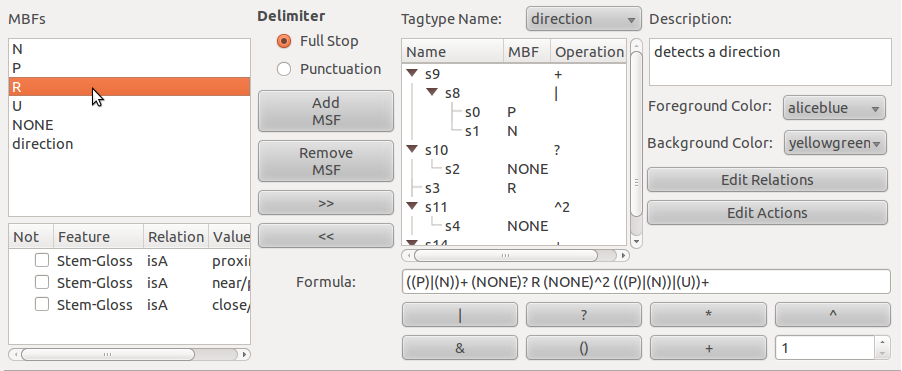
\includegraphics[width=\textwidth]{figures/mreedit}}}
  \caption{\framework tag type regular expression editor.}
  \label{f:sfe}
\end{figure}

\subsection{MBF match visualization}

%After defining the MBFs of the direction extraction task, 
%the user calls the MBF simulator from the {\tt Tagtypes} menu. 
%The snapshot in Figure~\ref{fig:mbftagger} shows 
The MBF match visualizer shows color sensitive text view, the tag list view, and the tag description view. 
%The color-sensitive text view shows the text with visualization of the MBF tag type matches. 
%The tag list view shows all tags.
%that are automatically or manually applied to the text. 
The tag description view presents the details of the selected tag along with 
the relevant tag type information.
%
The user can edit the tags using a context sensitive menus. 
\framework GUI also allows manual tag types and corresponding tags 
that are not based on morphological features.
This enables building reference corpora without 
help from the morphological analyzer.

\vspace{-1em}
\subsection{Tag type regular expression editor}

After interacting with the MBF editor, the user moves to 
specify the regular expressions. 
The MRE editor of Figure~\ref{f:sfe} allows the 
definition of an MRE tag type in a user friendly manner. 
The user first adds the required MBF formulae 
by selecting a label from ${\cal T}$ under MBFs. 
The Boolean formula of a highlighted tag type is shown in the table on the lower left pane. 
Each selected MBF is associated with an automatic name. 
The user can nest the MRE expression using a tree view of the MRE operations. 
The tree features the name, MBF, and operation for each sub-expression. 
%Moreover, a defined MRE is directly added to the MBF list enabling substitution and recursion 
%in formula definition.

%{\tt NONE} is a special tag type with no Boolean formula. 
%It tags all the words that are not tagged with any of the morphology-based Boolean tag types. 
%{\tt NONE} is defined by default and can be used to introduce flexibility and noise tolerance into the formula. 
%We previously defined this tag type in Section~\ref{sec:framework} and referred to it by $O$ (other).

%The regular expression editor enables the user to apply operations to the selected expressions. 
To specify a binary operation the user selects two sub-expressions and clicks the corresponding
operation button. 
%To do so, the user selects one or two expressions then selects an operation from the ones shown 
%in the lower left of the view. 
The operations include disjunction, conjunction, zero or one, sequence, zero or more, 
one or more, and up to a user defined constant.
The right pane shows a description of the tag type and a set of legend 
descriptors. 

%\[
%	(P|N)+~\mathit{O}?~R~\mathit{O^{\wedge}2}~(P|N|U)+
%\]
%In the direction task, we aim to build the expression shown above. 
%Thus we start by adding the MBFs $P$, $N$, $\textit{NONE}$, $R$, $\textit{NONE}$, $P$, $N$, and $U$. 
%We apply the required operations incrementally to build the final expression. 
%For example, we apply the disjunction ($|$) operation to the first $P$ and $N$ added, 
%then we apply the one or more ($+$) operation to the resulting sub-expression.
%We proceed as such to build the regular expression shown in Figure~\ref{f:sfe}. 
%Similar to the MBF tag type editor, the user specifies a set of legend descriptors for each MRE tag type.
%

\begin{figure}[tb!]
  \centering
  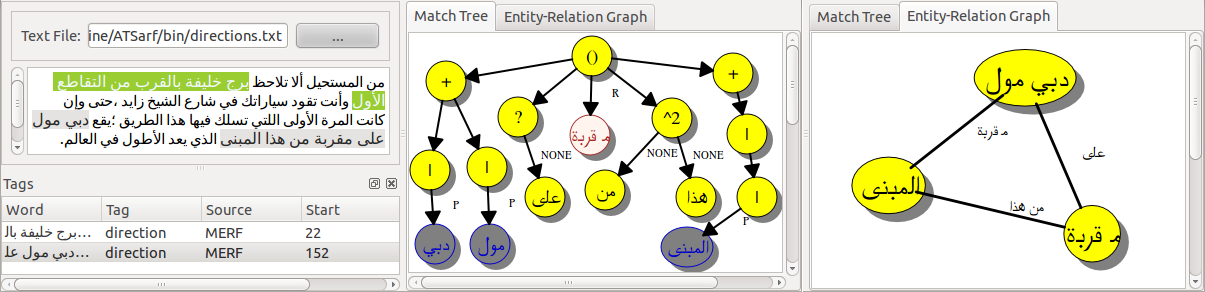
\includegraphics[width=\textwidth]{figures/treegraph}
  \caption{MRE annotated Text, MRE \major{matching parse tree}, and entity-relation graph}
  \label{fig:treegraph}
\end{figure}

\vspace{-1em}
\subsection{MRE match visualization}

While specifying an MRE the user can interact with the visualization and editor views
to make sure the MRE expresses the intent. 
The color-sensitive text view in Figure~\ref{fig:treegraph} shows 
the highlighted tag matches after the user called the MRE simulator using 
the {\tt Tagtypes} menu. 

The \major{matching parse tree} view shows the selected match in a graph view.
Figure~\ref{fig:treegraph} shows the \major{matching parse tree} of the direction task 
\RL{dby mwl `l_A mqrbT mn h_dA Almbn_A}(Dubai Mall is located near this building). 
%Leaf nodes show the match text, internal nodes show the operations, and edge labels shows the MBF tag type name.

%\begin{figure}[tb]
%  \centering
%  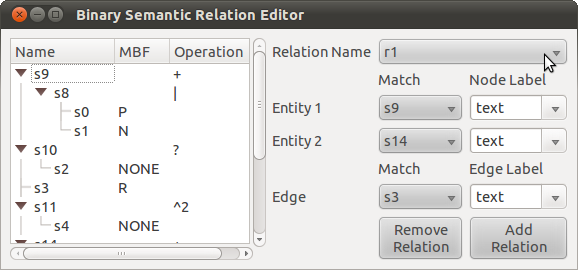
\includegraphics[width=0.5\textwidth]{figures/merfsreditor.png}
%\caption{\framework~relation editor}
%  \label{fig:relationeditor}
%\end{figure}

\subsection{User defined relation editor}

After the user is satisfied with the MRE matches, 
the user moves to define relations and code actions. 
The relation editor allows the user to define relations 
by specifying $\langle e_1,e_2,r\rangle$ tuples, 
where $e_1$ and $e_2$ denote source and destination entities, and $r$ denotes 
the label.
The editor shows the MRE tree and allows the user to select the sub 
expressions and select features 
of the matches of the sub expressions to define the three components of the relation. 

A snapshot of the GUI in 
Figure~\ref{fig:treegraph} shows in an interactive graph view
the entity-relation graph of the match of the user defined relation 
extracted from the \major{matching parse tree} of the MRE. 
%
In the computational action editor, an advanced user can 
enter C++ code and use the \framework API to program and process 
subexpression matches. 
%RE matches In order to add computational actions to an MRE sub-expression, 
%the user selects to edit the actions in the MRE tag type editor. 
%The view allows the user to specify the actions in a user friendly manner. 
%\framework provides the user with an API to access the sub-expression match features easily and define the pre-match actions. 
%The match features include the text, position, length, and numerical value if applicable, and morphological features for MBF matches. 
%\framework also enables the user to add C++ declarations and library includes.

\subsection{Analysis}

In the analysis view, the user provides 
two tag sets $R_1$ and $R_2$ and 
two tag type sets ${\cal T}_1$ and ${\cal T}_2$ as input. 
%The analysis view provides views of the differences between the tag types and 
%the tag sets.
%
The tag type difference view shows the text annotated in three panes: 
(i) the common tag types ${\cal T}_1 \cap {\cal T}_2$,
(ii) the tag types in ${\cal T}_1$ but not in ${\cal T}_2$, 
and (iii) the tag types in ${\cal T}_2$ and not in ${\cal T}_1$.
%
Similarly, the tag difference view shows $R_1\cap R_2$, $R_1/R_2$ and $R_2/R_1$
in addition to precision, recall and F-measure values. 
The user selects a predicate to compute the metrics from the following predicates:
(1) ``Intersection'': a tag from $R_1$ intersects in text with a tag in $R_2$,
(2) ``Exact'': a tag from $R_1$ exactly matches a tag in $R_2$,
(3) ``A includes B'': a tag from $R_1$ contains a tag from $R_2$, and
(4) ``B includes A'': a tag from $R_2$ contains a tag from $R_1$.
